\documentclass[these,auteur-annee,electrique, francais]{0_Hors_contenu/Apparences/udes-genie-demt-V1}
\usepackage[utf8]{inputenc}
\usepackage[hidelinks]{hyperref}

\usepackage{natbib} % for extra citation command
\usepackage{textcomp} % to use specific charactere

%package to include picture, figures, table %%%%%%%%%%%
\usepackage{graphicx}
\graphicspath{ {1_Bible/Photos/} }
%\usepackage{xprintlen}

\usepackage{rotating}
\usepackage{array,multirow}
\usepackage{booktabs}
\usepackage{tabularx}
%%%%%%%%%%%%%%%%%%%%%%%%%%%%%%%%%%%%%%

%change internal link from red to black - especially for ToC
\usepackage{hyperref}% http://ctan.org/pkg/hyperref
\hypersetup{%
  colorlinks = true,
  linkcolor  = black
}

%change text, sections, .. colors
\usepackage[dvipsnames]{xcolor}


%Custom things units %%%%%%%%%%%%%%%%%%
\usepackage{siunitx}
\let\DeclareUSUnit\DeclareSIUnit
\let\US\SI
\DeclareUSUnit\inch{\mydprime}
%%%%%%%%%%%%%%%%%%%%%%%%%%%%%%%%%%%%%%%

%%%
%%%
% Fichier pour les nouvelles commandes
%%%
%%%




%%
% Commandes pour les inclusions de texte ou de figures.
%%
\newcommand{\Adams}[1]{2_Fiche_lecture/Articles/#1-Adams/}

\MotsCles{Haptique, Neuroscience, Systéme somatosensoriel}
\FichierResume{0_Hors_contenu/Informations/resume}
\FichierRemerciements{0_Hors_contenu/Informations/merci}
\FichiersBibliographiques{0_Hors_contenu/Informations/references}

\Dedicace{Aux dauphins}
\FichierLexique{0_Hors_contenu/Informations/lexique}
\FichierSymboles{0_Hors_contenu/Informations/symboles}
\FichierAcronymes{0_Hors_contenu/Informations/acronymes}

\begin{document}
%\tableofcontents %generate and print ToC

\part{Bible Haptique\\ R\'esum\'e des connaissances}

	\chapter{SENS, SENSATION, PERCEPTION}

	\input{1_Bible/Chapters/1_Sens_Sensation_Perception/1.Les_Sens}
	\section{Distinction entre sensation et perception}
La sensation est la stimulation des récepteurs sensoriels qui produisent des potentiels d’actions que le cerveau interprètera. Une sensation se produit lorsqu’un organe sensoriel absorbe l’énergie provenant d’un stimulus physique venant de l’environnement extérieur. Les récepteurs sensoriels convertissent cette énergie physique en  potentiel d’action et les transmettent au cerveau via les nerfs.\par
La perception c’est quand le cerveau organise les informations sensorielle et les traduis/interprète en quelque chose significatif, qui a du sens ou qui peut être rationalisé. De plus, la perception est comment quelqu’un reçoit ce sentiment ou cette pensé, et y donne sens à travers la mémoire et l’émotion. La perception est principalement « comment » le cerveau interprète une sensation. L’information est obtenue à travers la collection, réception, transmission et mécanisme de codage.\par
Sensation et perception se complémentent l’un et l’autre pour donner du sens à notre expérience, mais restent deux complétement différente moyen de comment on interprète notre monde.\par
La perception est propre à chaque individu - différences intersujets, mais peut aussi varié au sein d’une même personne (i.e. des sensations identiques peuvent entraîner des perceptions différentes) - différences intrasujets. Ces différences viennent du fait que ce que nous percevons de notre environnement dépend de nos connaissances, de nos humeurs, de nos motivations, etc. Il arrive aussi qu’à certains moments, nos perceptions puissent dépasser les données sensorielles reçues, la perception va plus loin que la sensation. Exemple perception : un objet qu’on regarde peut nous apparaître chaud, rugueux, lourd.\par



	\section{Cross-modalité et congruence}
Quand deux sensations venant d’un système sensoriel différent, arrivent au SNC, l’information est traitée comme un tout afin de donner lieu à une unique perception. On défini alors l’information provenant d’un système sensoriel comme une modalité et on dit que la perception résultante de plusieurs modalité est cross-modale.\par
Les informations provenant de deux modalité différentes peuvent être congruente (cohérente) et ainsi renforcé la perception. Dans le cas inverse les informations sont contradictoires et alors la perception sera biaisée vers l’une ou l’autre des modalités. Cette contradiction peut aussi donner lieu à des illusions (voir section correspondante).\par


	\section{Illusion}
Illusion Haptique --- \url{https://lejournal.cnrs.fr/articles/lillusion-tactile-une-revolution-en-marche}\par

\subsection{ \textit{Fishbone illusion}}
Soit une surface découpé en trois partie : coté droit, milieu, coté gauche. Si les coté droit et gauche de la surface ont une texture plus rugueuse que le milieu, lorsque quelqu’un déplace sont doigt le long de la surface, il percevra le milieu de la surface à un renfoncement/creux.\par

\subsection{ \textit{Bump/hole illusion}}
Lorsque le doigt parcourt une surface, une information kinesthetic de creux ou de bosse, sera perçu de la même manière par une même personne.\par

\subsection{ \textit{Cutaneous Rabit illusion (saltation)}}
Original : Une série de courts pulses délivrés successivement à trois différente position sur la peau sont perçu comme un seul et unique stimulus bougeant progressivement le long de la peau. Comme si un petit lapin sautillée progressivement du premier au troisième stimulateur.\par
Réduit : 3 stimulation à 2 location, une des stimulations sera perçu au milieu des deux locations.\par
Exemple d’expérience :
\begin{itemize}
	\item Original : marche mieux avec 3-6 « tapements » et un intervalle inter-stimuli entre 20-250ms;
	\item Zone : 2.28cm2 sur l’index et 145.7cm2 sur l’avant bras.
\end{itemize}

\subsection{Illusion du peigne --- \textit{comb illusion}}
Lors d’une succession de stimuli de cisaillement, un stimulus de cisaillement plus « fort » peut induire l’illusion de la présence d’un pic.\par

\subsection{\textit{Apparent motion(effet phi)}}
L’illusion d’un déplacement continu peut être donné au travers de tapements successifs le long d’un trajet discontinu. La durée des tapements et l’intervalle inter-stimuli sont les paramètres principaux permettant la réalisation de cette expérience. Exemple d’expérience :
\begin{itemize}
	\item Tapement durée : 25-400ms;
	\item Meilleur avec tapement de 100ms et intervalle inter-stimulus de 70m;
	\item Intervalle 320ms avec 3 tapements et intervalle 20ms avec 12 tapements.
\end{itemize}

\subsection{Phantom-Funneling illusion}
Quand de bref stimuli sont presenté simultanément à différents points proche sur la peau, ils sont souvent perçus comme un unique stimulus central plutôt qu’une sensation phasique aux différentes positions. C’est comme si le stimulus tactile était « cheminée » vers une position centrale à laquelle le stimulus était perçu plus fort qu’à la position individuelle de stimulation.\par
Exemple d’expérience :
\begin{itemize}
	\item 3 stimulateurs sur l’avant bras (espacé de 30mm) à localisé dans une bande de 20mm autour du stimulateur du milieu. (robustesse: 80\%);
	\item 2 stimulateurs à point “phantom” au milieu, la position peut être variée vers un stimulateur ou l’autre en faisant varié le ratio d’amplitude des stimulateurs;
	\item Intensité au point « phantom »: $A_phantom^2= A_point1^2+A_point2^2$.
\end{itemize}

\subsection{Tau effect}
Le tau effect représente la dépendance temporelle de la perception des distances. Par exemple soit 3 stimuli successif sont présenté aux locations A,B et C. Si ces locations sont espacé tel que la distance AB soit 2 fois plus grande que la distance BC et que le temps entre le stimulus en A et celui en B soit deux fois plus lent qu’entre le stimulus B et C. Alors la distance AB sera perçu 4 fois plus grande que BC.\par
Cette illusion fonctionne aussi pour des stimuli mobile : Un stimulus rapide sera perçu comme parcourant une distance plus courte qu’un stimulus lent faisant le même parcourt.\par
Dans d’autre modalité, la dépendance spatial de la perception des durations (effet kappa) a été observé, mais ne semble pas existé pour le sens tactile.\par
Exemple d’expérience :
\begin{itemize}
	\item 3 points illusion : Meilleur si le ratio temps est inférieur à 4 :1, marche pour des distances allant de 30 à 85mm sur l’avant bras et des intervalle de temps inter-stimuli variant de 200 à 500ms;
	\item Stimulus mobile : Un stimulus rapide (2500mm/s) et un stimulus lent (10mm/s), la distance sera réduit de 50\%. Ne marche pas pour des stimuli de 50-200mm/s.
\end{itemize}







	\chapter{SENSATION TACTILE}
Ici nous présentons le chemin de l’information et détaillons les points clé dans des sections séparé.\par

\section{Cheminement de l’information}
La zone 3b est seulement à 3 synapses de la fibre sensorielle. (via le cuneate nucleaus and the talamus).\par
\begin{figure}[!h]
	\centering
	\includegraphics[width=10cm]{1_Bible/Photos/Biology/chemin.jpg}
	\caption{Cheminement de l’information}\label{chemin_info}
\end{figure}



\section{Mécanique du contact}

\subsection{Définition des termes}
Force : Dans la mécanique du point, une force est représenté par une direction (vecteur) et une amplitude (scalaire). Dans la mécanique du solide, le concept est étendu à une matrice 3x3 où chaque ligne représente les forces soumises sur les faces du cube élémentaire. On parle alors de tenseur de force. Les éléments sur la diagonale du tenseur sont appelés les efforts normaux, et les autres les efforts tangentiels. Dans certain cas, une matrice du moment peut être définie pour décrire les forces de rotations.\par
Déformation : La différence de géométrie entre l’état l’initiale et l’état qui suit l’exercions  du tenseur de force peut être définie avec un tenseur de déformation.\par
Élasticité : Décris la capacité d’un matériau de résister une force qui lui est appliqué. Exprimé avec le coefficient de Young.\par
Viscosité : Décris la composante temporelle qui lie application d’une force et déformation.\par
Compressibilité : Décris la capacité d’un matériau à se comprimer. Exprimé avec le coefficient de poisson.\par

….Distinction entre force normale, pression ; glissement, effort tangentiel; contraint, effort; tenseur de déformation…\par
…Distinction entre force et pression\par

\subsection{Contact statique}
Loi de hooke : Relie les deux grandeurs force et déformation\par
Contact Hertzien : Décrie les déformations\par

\subsection{Contact dynammque}
...

\subsection{Déformation local}
...

\subsection{Déformation distante -- Propagation des ondes}
Lors d’un stimulus tactile, des ondes se propagent à la surface de la peau, dans les couches inférieures de la peau et dans les organes. De ce fait les MRs distant du point de contact sont aussi stimulé par le contact. En plus de MRs cutanée, les MRs au niveau des muscles, tendons et articulation sont aussi stimulé. Il a été mis en évidence, que selon l’interaction tactile, le motif de propagation d’ondes sera différent. Ce qui alimentent l’hypothèse que ces ondes sont pris en comptent lors de l’interprétation d’un stimulus. Par exemple, lors d’un toucher d’exploration, la texture de la surface va créer un motif d’ondes particulier qui se fera sentir jusqu’au poignet, où des PC récepteurs pourront encodé la texture et ainsi permettre l’indentification de la texture parcouru.\par

Qu’est ce qui est pondérant, la propagation de la vibration : dans la peau, dans les os, dans les tendons ?\par



\section{Mécano-transduction}
Sous la stimulation, les mécanorécepteurs émettent des potentiels d’action le long des nerfs afférents et en direction du CNS. Le procédé par lequel une excitation sensorielle (ici mécanique) donne lieu à un potentiel d’action est nommé mécano-transduction. Ce procédé a fait l’objet de différentes études et a été modélisé.\par
Chaque mécanorécepteur encode la déformation mécanique en un potentiel d’action d’une manière différente. Il est a noté aussi que chaque mécanorécepteur semble sensible à différents types de stimuli (voir correspondant sous-partie).\par

\subsection{PC}
...

\subsection{RA}
...

\subsection{SAI}
...

\subsection{SAII}
...

\subsection{Fibre de type C}
...

\subsection{Exemple de modélisation}
...



\section{Séquence de potentiel d’action (spike train)}
Les mécanorécepteurs produisent une séquence de potentiel d’action dont l’amplitude et la fréquence est propre à la caractéristique de la sensation. La séquence de potentiel d’action peut alors être interprété comme l’encodage de la sensation.\par
\begin{figure}[!h]
	\centering
	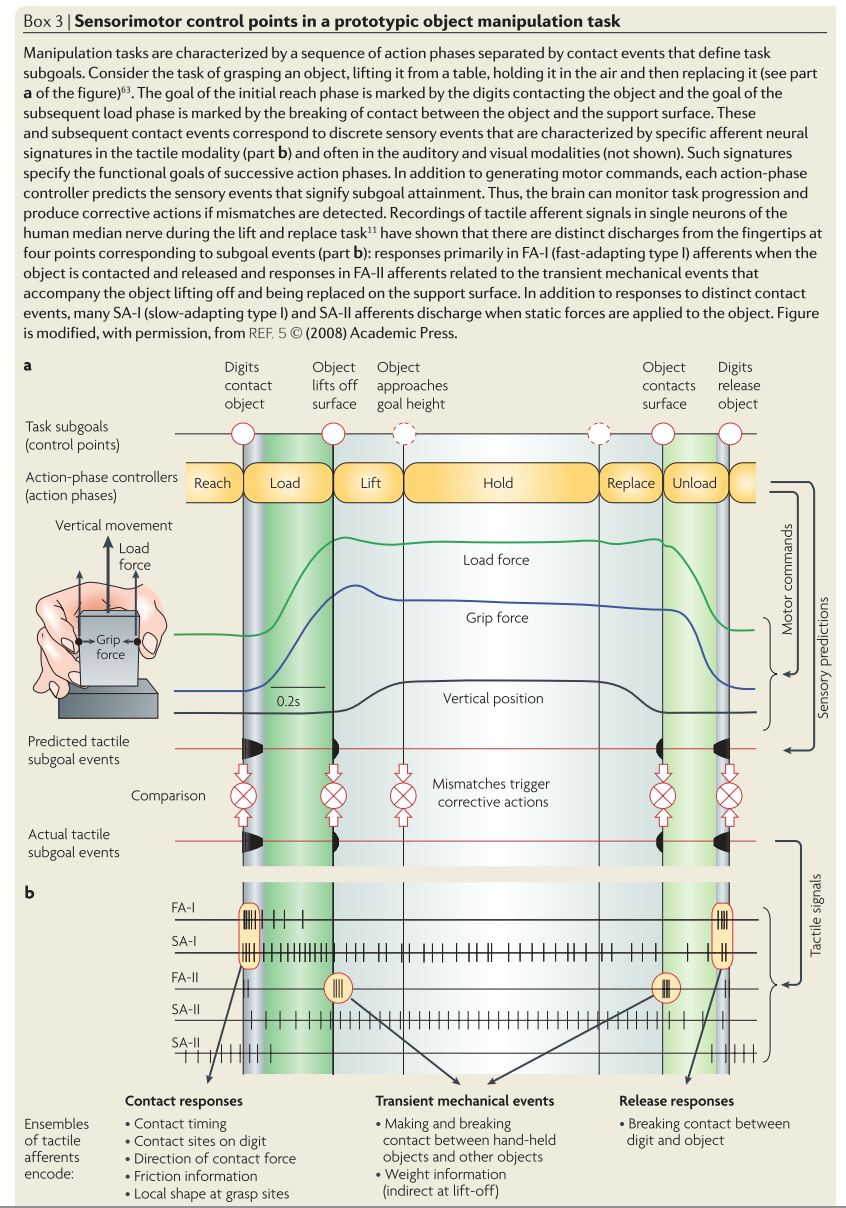
\includegraphics[width=12cm]{1_Bible/Photos/Biology/potentiel_daction.png}
	\caption{Exemple de séquence de potentiels d'action lors d'une tache de manipulation}\label{potentiel_daction}
\end{figure}



\section{Mesure Psychophysique}
Le sens du toucher peut sentir divers stimuli tactile. Néanmoins, comme tout récepteur/senseur, il ne peut sentir qu’à partir d’une intensité minimum (seuil de perception) et ne peux distinguer qu’une différence minimale entre deux intensités (seuil de discrimination). Ces caractéristiques peuvent être mesuré et quantifié grâce à divers expériences  psychophysiques (exemple tableau ci-dessous).\par
\begin{table}[!h]
	\caption{Seuil de perception (résolution) et seuil de discrimination (weber fraction) pour différent types de sensation (stimulus dimension)}
	\label{tab_mesure_psycho}
	\centering
	\begin{tabular}{|p{5cm}|p{5cm}|p{4cm}|}
		\hline \rule[-7pt]{0pt}{20pt}
		Dimension de la stimulation&Résolution&Fraction de Weber(\%)\\
		\hline
		\rule[-7pt]{0pt}{20pt}Texture de surface (rugosité)& 0.06... & 5-12\% \\
		\hline
		\rule[-7pt]{0pt}{20pt}...&...& ...\\
		\hline
		\rule[-7pt]{0pt}{20pt}...&...&...\\
		\hline 
		\rule[-7pt]{0pt}{20pt}...&...&...\\
		\hline
		\rule[-7pt]{0pt}{20pt}...&...& ...\\
		\hline
		\rule[-7pt]{0pt}{20pt}...&...&...\\
		\hline 
		\rule[-7pt]{0pt}{20pt}...&...&...\\
		\hline
		\rule[-7pt]{0pt}{20pt}...&...& ...\\
		\hline
		\rule[-7pt]{0pt}{20pt}...&...&...\\
		\hline 
		\rule[-7pt]{0pt}{20pt}...&...&...\\
		\hline
		\rule[-7pt]{0pt}{20pt}...&...& ...\\
		\hline
		\rule[-7pt]{0pt}{20pt}...&...&...\\
		\hline 
		\rule[-7pt]{0pt}{20pt}...&...&...\\
		\hline
		\rule[-7pt]{0pt}{20pt}...&...& ...\\
		\hline
		\rule[-7pt]{0pt}{20pt}...&...&...\\
		\hline
	\end{tabular}
\end{table}
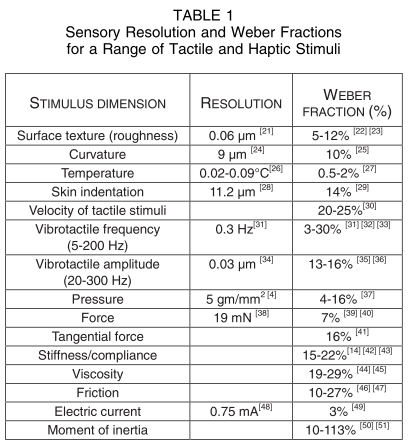
\includegraphics[width=10cm]{1_Bible/Photos/Biology/tab_seuil.png}

\subsection{Seuil de perception -- \textit{Threshold}}
...

\subsection{Seuil de discrimination -- \textit{JND}}
...

\subsubsection{Seuil de discrimination spatiale}
La méthode du seuil de discrimination spatiale consiste à déterminer la distance minimale qu’un sujet (les yeux fermés) n’arrive plus à distinguer les deux pointes qui lui appliqué sur la peau. En fonction des différentes partie du corps, le seuil – entre ressentir les deux pointes et le passage ou le sujet ne pense qu’il n’y en a plus qu’une. Zones plus sensible de que d’autre. Les MRs ne sont pas réparti de la façon sur le corps, la densité est différente.\par
\begin{figure}[!h]
	\centering
	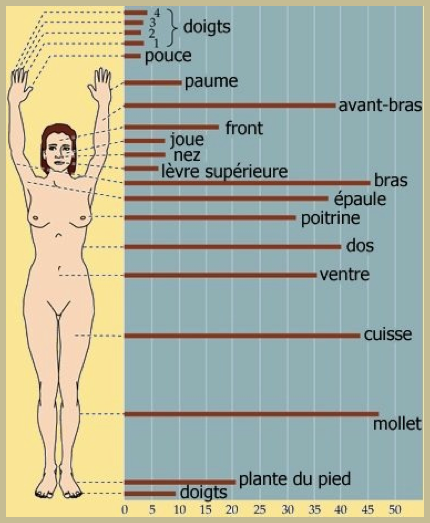
\includegraphics[width=10cm]{1_Bible/Photos/Biology/discrim_spatiale.png}
	\caption{Tests des deux points}\label{discrim_spatiale}
\end{figure}
Les parties les plus sensibles sont les mains, le visage et les doigts de pieds.

\subsection{Méthode de mesures psychophysique}
...

\subsubsection{Méthode classique}
...

\subsubsection{Théorie de la détection du signal}
...






	\chapter{PERCEPTION TACTILE}
Sens du toucher : (déf) système qui peut mesurer une propriété donnée d’un objet ou d’un phénomène, au travers d’un contact physique entre le système et l’objet. [Lederman SJ. Tactual Perception]\par
Le sens du toucher pour certains animaux est primordial. Les araignées sont très sensibles au toucher mais ne voient pas la lumière, l’obscurité et les formes basiques [Barth’2016…]. Les araignées apprennent plus sur leur environnement en ressentant les vibrations qu’en utilisant leurs yeux. Elles arrivent à faire la distinction en les différentes vibrations (insert dans la toile, vent qui souffle, autre araignées sur la toile, …).\par
Diap presentation\par
Le sens du toucher chez les mammifères et humains :\par
…Les Mammifères […]\par
…Le premier sens développé chez le fétu – au bout de 7 semaines, haptonomie - \par
Sens de nature complexe et non intuitive. Ce n’est pas une simple transduction d’une propriété physique en un signal électrique. Elle peut prendre plusieurs formes de la détection d’une texture, d’une forme, d’une blessure, d’un échange et autre. Les dernières avancées dans le domaine de l’haptique, des neurosciences cognitives et psychologiques.\par
Par rapport au sens de l’ouïe ou de la vue, le toucher reste encore une quantité définie. Dans les prochains paragraphes, un état de l’art sur la mécanique de la peau, les systèmes mécanorécepteurs de la peau jusqu’au système somatosensoriel va être établi à partir des dernières études faites en haptique.\par


\section{Procédure d’exploration}
Pour satisfaire ces besoins la peau doit être capable distingue et faire émerger différentes propriétés. Pour ce faire. La main interagi avec un objet/surface selon plusieurs méthodes. Ces méthodes recensé dans une étude de Lederman et Klatzy sont nommé « exploratory procedure » or EP for short (Lederman \& Klatzky 1987):\par
\begin{figure}[!h]
	\centering
	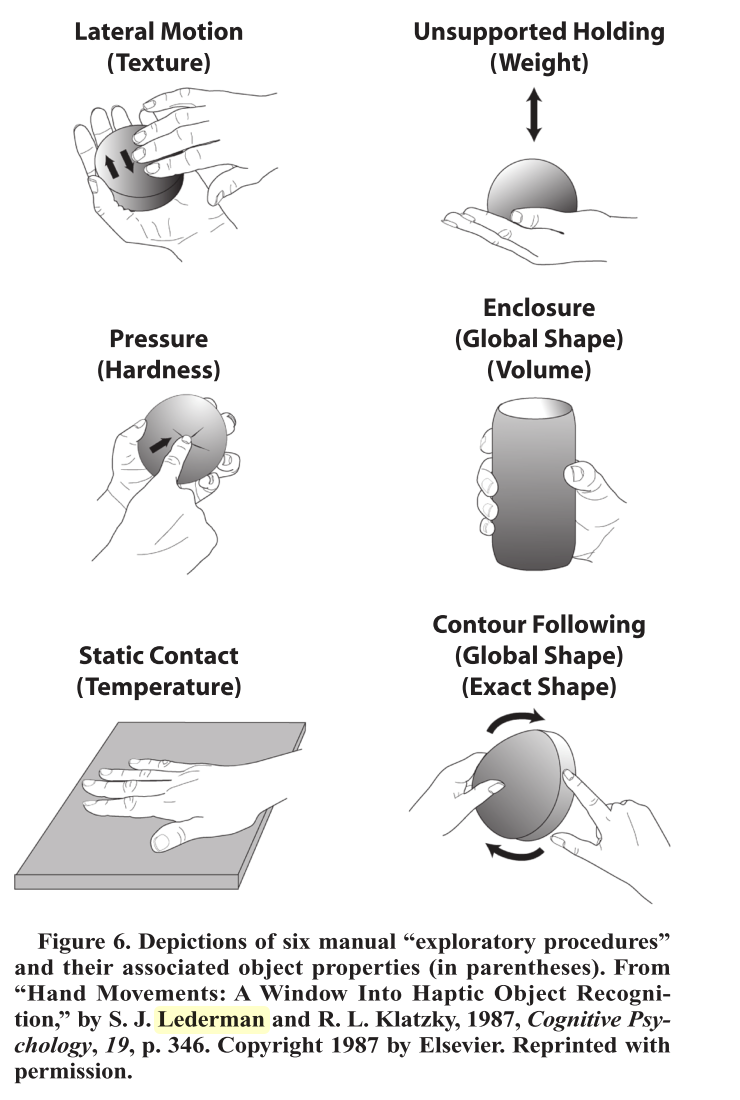
\includegraphics[width=7cm]{1_Bible/Photos/Psychology/proc_explo.png}
	\caption{Procédure d’exploration [] }\label{proc_explo}
\end{figure}



\section{Dimension du toucher}
Les EP, vu précédemment, servent notamment à renseigner sur la nature de l’objet/surface manipuler, qui sont caractérisé par les grandeurs physique et psychophysique suivante (Okamoto et al. 2013):
\begin{itemize}
	\item Texture;
	\begin{itemize}
		\item Rugueux/lisse;
		\begin{itemize}
			\item Macro-echelle (coarse);
			\item Micro -echelle (fine);
		\end{itemize}
		\item Dur/mou;
		\item Friction;
		\begin{itemize}
			\item Humide/sec;
			\item Glissant/collant;
		\end{itemize}
	\end{itemize}
	\item Température : Chaud/Froid;
	\item Forme : global/exact;
	\item Poids.
\end{itemize}
La texture regroupe plusieurs dimension et non seulement des information de rugosité. (voir liste au dessus).\par
Dualité de la perception de la rugosité : La rugosité d’une surface est perçu à deux échelles : Une macro-échelle, de l’ordre du millimetre et une micro-echelle de l’ordre du micrometre (voire nanometre). Cette difference d’échelle s’explique par les mecanisme du toucher qui encode la rugosité. La macro echelle vient du fait que les MR SA1 encode les informations de rugosité localement, là où peau et surface font contact. De ce fait, les limite de perceptions dépendent de l’acuité spatiale du sens du toucher. (threshold autour de 1mm). La micro-echelle dépend des MR PC qui encode les vibration créent par le doigt parcourant la surface. Ces vibrations se propagent dans tout le doigt, la paume des mains et vont même jusqu’au poignet. Des détails aussi fin que de qq centaine de nanomètre peuvent induire de telle vibration.\par
…Les parties les plus sensibles de notre corps humain sont les parties telles que : la figure, l’arrière de la nuque, les mains, le haut du bras, le torse, entre les jambes et la plante des pieds.\par
Et les changements d’état de celui-ci, glissement d’un objet, caresse,…\par
Le système somatosensoriel traite les données spatiotemporelles provenant des mécanorécepteurs [glissement, vibration], thermorécepteur [température] et nocicepteur [blessure] compris dans la peau.\par




\section{Taux de transfert d’information tactile}
...



\section{Types de toucher}
Outre tous les caractéristiques biologiques de la peau et les informations qu’il est possible d‘en retirer quant à son importance dans la sensation d’une surface/d’un objet (i.e.: la souplesse/dureté de la surface de contact, sa température, sa texture, sa forme, etc.), il est intéressant de noter que notre perception se découpent en différents types de toucher, aux caractéristique différentes (exemple : récepteur stimulé). En tout on peut distinguer jusque quatre type de toucher : de manipulation, d’exploration, communicatif et protectif.\par

\subsection{Toucher de manipulation}
Type de peau : glabre\par

Le toucher de manipulation est spécifique à la peau glabre est aussi celui qui a été le plus étudié.

\subsection{Toucher d’exploration}
Type de peau : Glabre ; et Poilu pour la navigation\par
Le toucher d’exploration est…

\subsection{Toucher communicatif}
Type de peau : Poilu\par
Le toucher communicatif est …

\subsection{Toucher protectif}
Type de peau : Poilu\par
Le toucher est …









	\chapter{LES TECHNOLOGIES HAPTIQUES}
Retrouver les photos en HD !\par

\section{Systèmes récepteurs}
\subsection{Ecran tactile}
\subsection{Peau tactile}
\subsection{CNC}
\subsection{CNP}



\section{Systèmes acteurs}

\subsection{Interfaces à retour de force}
\begin{figure}[!h]
	\centering
	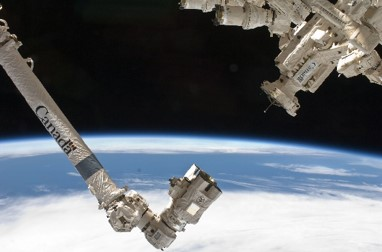
\includegraphics[width=6cm]{1_Bible/Photos/Apparatus/bras_ca.jpg}\hspace{2cm}
	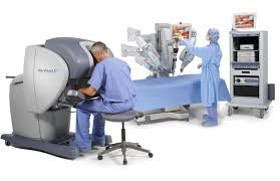
\includegraphics[width=6cm]{1_Bible/Photos/Apparatus/da_vinci.jpg}
	\caption{Interfaces à retour de force : a) ... }\label{int_retourf_1}
\end{figure}
\begin{figure}[!h]
	\centering
	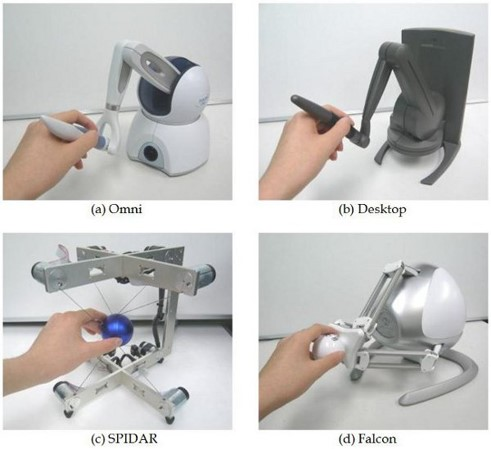
\includegraphics[width=7cm]{1_Bible/Photos/Apparatus/falcon.jpg}
	\caption{Interfaces à retour de force : a) ... }\label{int_retourf_2}
\end{figure}	
\begin{figure}[!h]
	\centering
	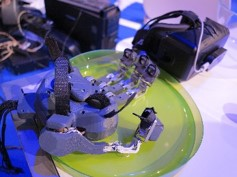
\includegraphics[width=4cm]{1_Bible/Photos/Apparatus/cea_gant_1.jpg}\hspace{1cm}
	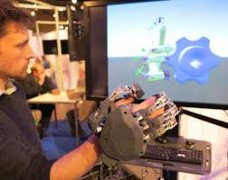
\includegraphics[width=4cm]{1_Bible/Photos/Apparatus/cea_gant_2.jpg}\hspace{1cm}
	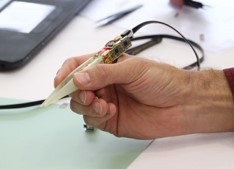
\includegraphics[width=4cm]{1_Bible/Photos/Apparatus/pince_isir.jpg}
	\caption{Interfaces à retour de force: a) ... }\label{int_retourf_3}
\end{figure}

\subsection{Interfaces à retour tactile}

\subsubsection{Par contact direct -- ''\textit{tangible}''}
\begin{figure}[!h]
	\centering
	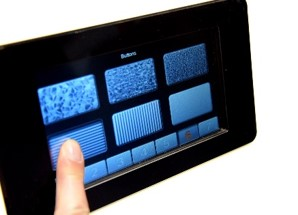
\includegraphics[width=6cm]{1_Bible/Photos/Apparatus/tangible_cea_e-t.jpg}\hspace{2cm}
	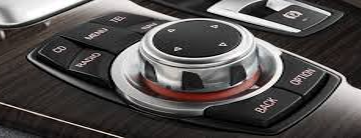
\includegraphics[width=6cm]{1_Bible/Photos/Apparatus/tangible_cea_magneto.png}
	\caption{Interfaces à retour tactile par contact direct: a) ... }\label{int_retourd_1}
\end{figure}
\begin{figure}[!h]
	\centering
	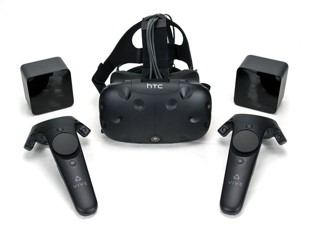
\includegraphics[width=6cm]{1_Bible/Photos/Apparatus/tangible_vive.jpg}\hspace{2cm}
	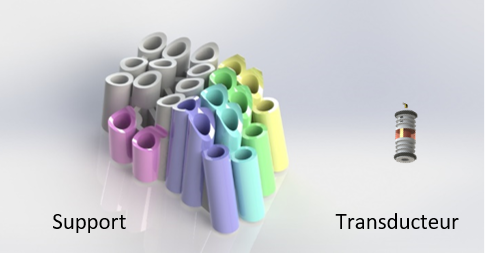
\includegraphics[width=6cm]{1_Bible/Photos/Apparatus/tangible_com_hapt.png}
	\caption{Interfaces à retour tactile par contact direct: a) ... }\label{int_retourd_2}
\end{figure}

\subsubsection{Par contact indirect -- ''\textit {mid-air}''}
\begin{figure}[!h]
	\centering
	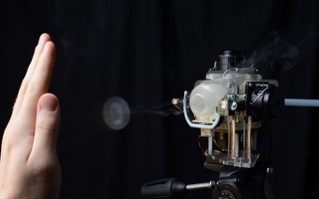
\includegraphics[width=6cm]{1_Bible/Photos/Apparatus/mid_air_disney.jpg}\hspace{2cm}
	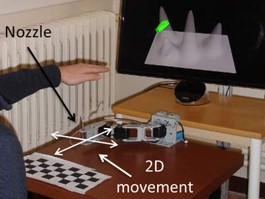
\includegraphics[width=6cm]{1_Bible/Photos/Apparatus/mid_air_jet.jpg}
	\caption{Interfaces à retour tactile par contact indirect : a) ... }\label{int_retourid_1}
\end{figure}
\begin{figure}[!h]
	\centering
	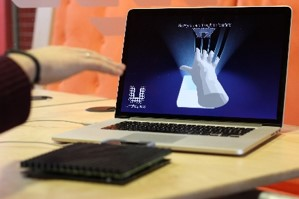
\includegraphics[width=7cm]{1_Bible/Photos/Apparatus/mid_air_ultrahaptics.jpg}
	\caption{Interfaces à retour tactile par contact indirect : a) ... }\label{int_retourid_2}
\end{figure}	




	\chapter{LA PEAU}




	\chapter{LE SYSTÈME NERVEUX}

On distingue le système nerveux central (SNC) et le système nerveux périphérique (SNP).\par


	

\part{Fiches des articles}
	\chapter{Biom\'{e}canique}
		
\section {Finger pad friction and its role in grip and touch (2012) \textit{Adams et al.} }
	Le papier fait un \'{e}tat de l'art de la litt\'{e}rature sur la friction ayant lieu au point de contact entre doigt et surface.
	Le papier est divis\'{e} en 4 partie: Surface de contact, occlusion, l'\'{e}volution du slip dans la r\'{e}gion de contact et l'influnce de la vitesse de glissement.\\
	
	
	\input{\Adams{2012}Subsections/contact_area}
	\input{\Adams{2012}Subsections/Occlusion}
	\input{\Adams{2012}Subsections/Evolution_of_slip_in_the_contact_region}
	
	

\appendix

\chapter{APP TEST}


\end{document}
